\section{Specific Requirements}
\subsection{Functional Requirements}


\subsubsection{Use Cases Diagrams}
In this section, we will provide use case diagrams. Then, for each use case, we will provide a detailed description and a sequence diagram.
\\
\textbf{Note}: in the following diagrams, it is the user who initiates the use case

\vspace{3px}
\begin{figure}[H]
    \centering
    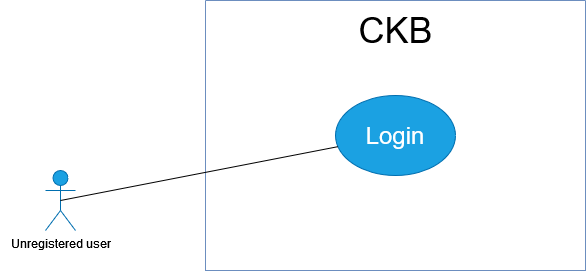
\includegraphics[scale=0.6]{src/uc_diagrams/unregistered_user.png}
    \caption{Unregistered user use case diagram}
\end{figure}

\vspace{3px}
\begin{figure}[H]
    \centering
    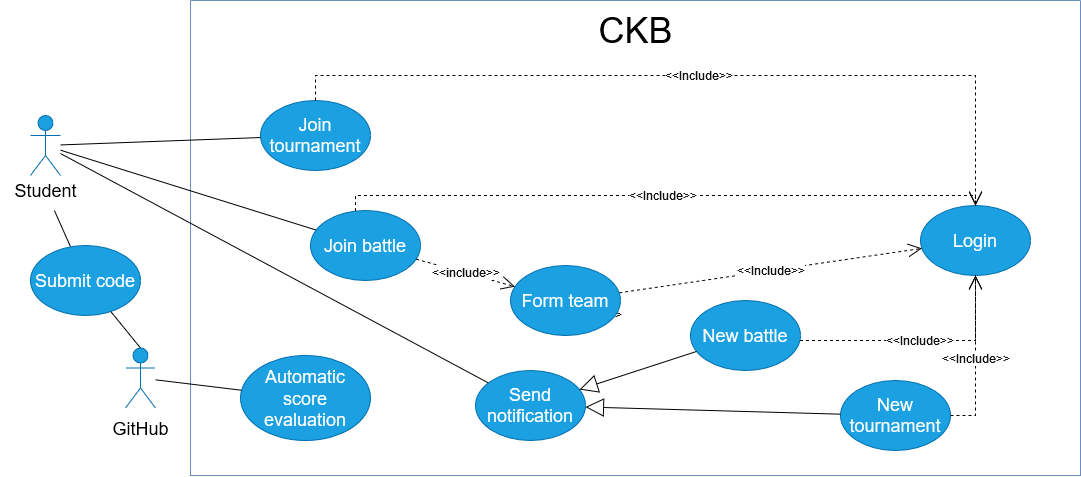
\includegraphics[width=\textwidth]{src/uc_diagrams/student.png}
    \caption{Student use case diagram}
\end{figure}

\vspace{3px}
\begin{figure}[H]
    \centering
    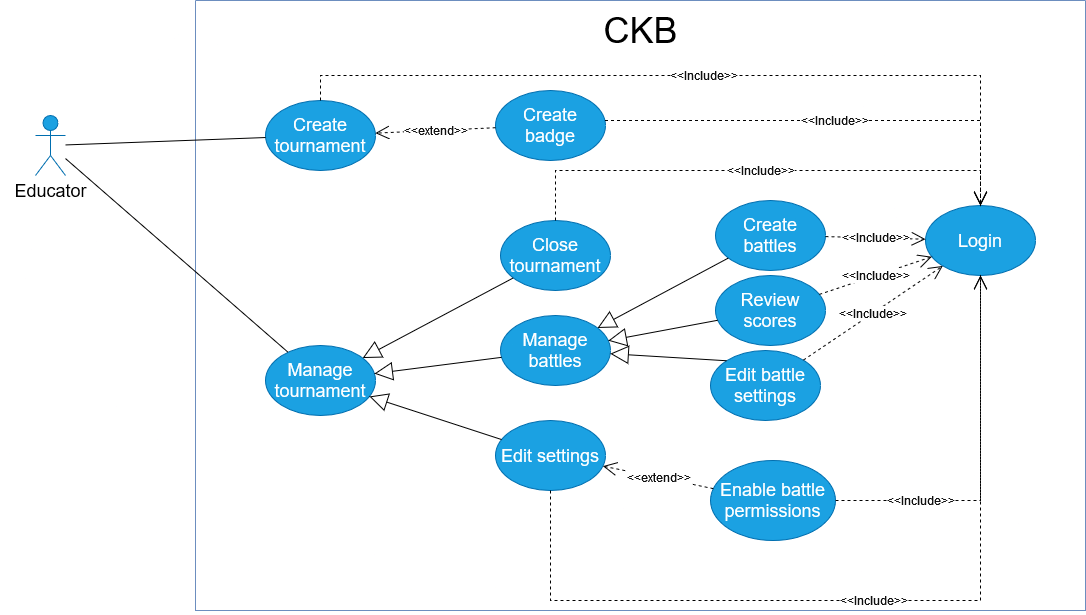
\includegraphics[width=\textwidth]{src/uc_diagrams/educator.png}
    \caption{Educator use case diagram}
\end{figure}

\vspace{3px}
\begin{figure}[H]
    \centering
    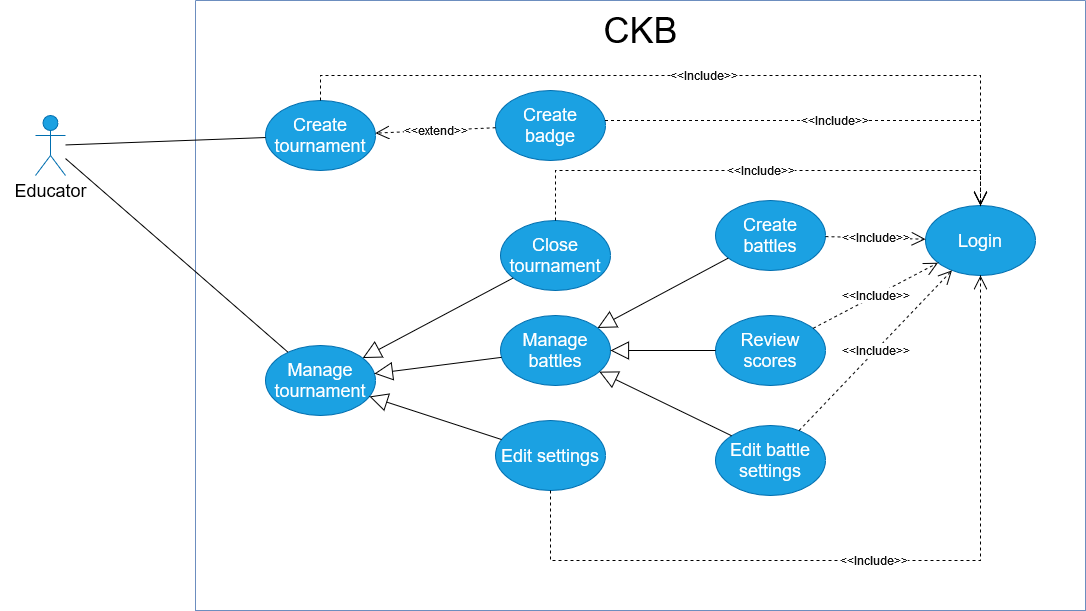
\includegraphics[width=\textwidth]{src/uc_diagrams/generic_user.png}
    \caption{Generic user use case diagram}
\end{figure}

\newpage


\subsubsection{Use Cases}
In the following use cases and sequence diagrams, the system is to be seen as black box interacting with the world.
\usecase
{
    \begin{figure}[H]
        \centering
        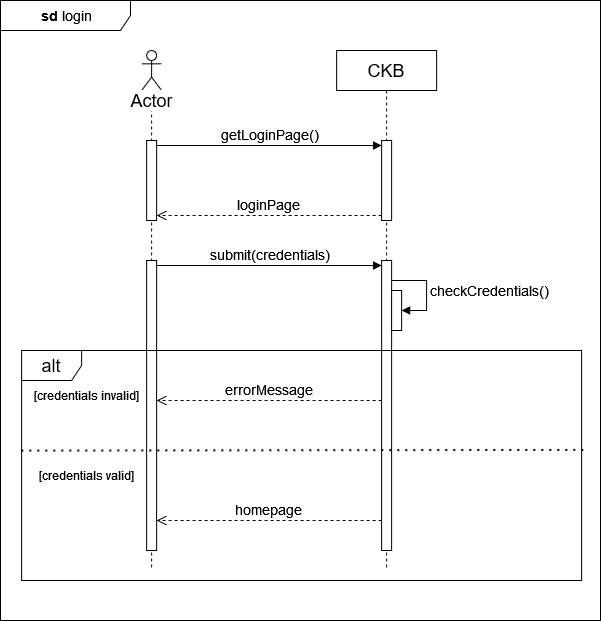
\includegraphics[width=\textwidth]{src/sequence_diagrams/sqlogin.png}
    \end{figure}
}
{1}
{Login}
{User}
{The actor is already registered in the system}
{
    \begin{enumerate}
        \item User requests the Login Page
        \item The system shows the Login Page to user
        \item User inserts credentials and sends them to the system
        \item The system processes the information and shows a success message redirecting the user to the homepage
    \end{enumerate}
}
{User is logged and the homepage is displayed}
{
    \begin{itemize}
        \item A wrong username or password is submitted
    \end{itemize}
}
{
    In case of exception, a human-readable message will be returned by the system.
}

\usecase
{
    \begin{figure}[H]
        \centering
        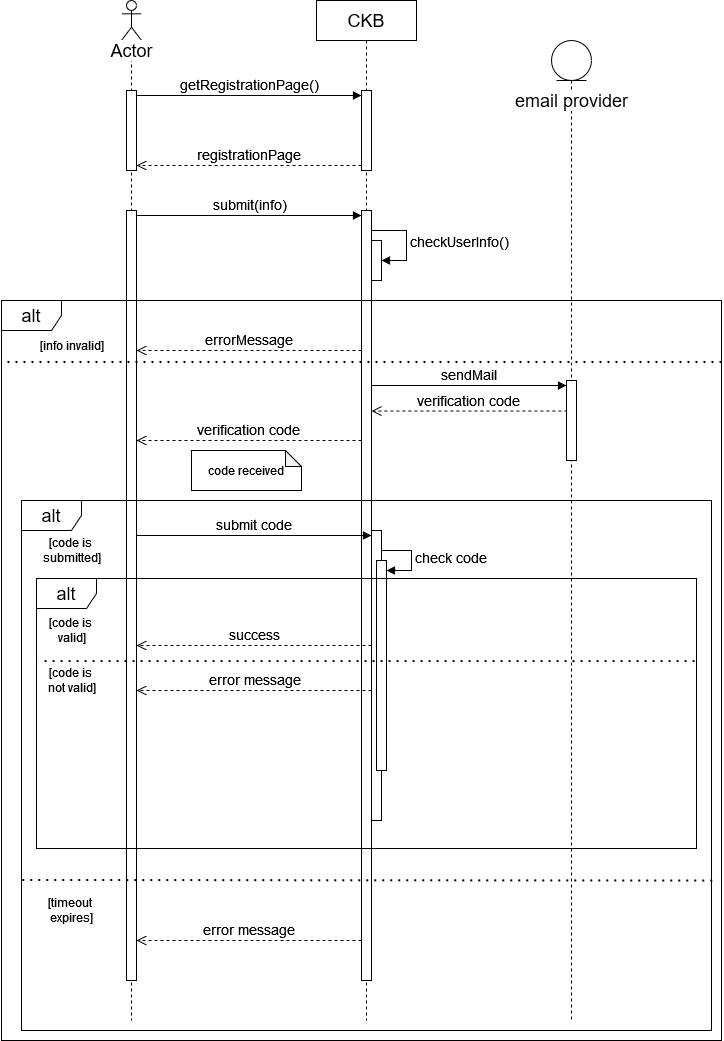
\includegraphics[width=\textwidth]{src/sequence_diagrams/register.png}
    \end{figure}
}
{2}
{User registration} % name
{User, Email provider} % actor
{User clicks 'Sign Up' in the homepage} % entry condition
{ % event flow
    \begin{enumerate}
        \item The system sends user the registration form
        \item User enters email, username password and academic status. Then, submits the data after reading and accepting the Privacy Policy and the Terms of Service
        \item The system sends an email with a secret verification code to Email provider
        \item Email provider receives the email and notifies user
        \item User submits the verification code in the email
        \item The system processes the provided information and displays a success message
    \end{enumerate}
}
{A new account is created} % exit condition
{ % exceptions
    \begin{itemize}
        \item A required registration field is missing when the form is submitted
        \item The username is not available
        \item A wrong verification code is submitted
        \item The timeout for verification expires
    \end{itemize}
}
{ % notes
    All the exceptions above will notify operator with a human-readable message and the system asks to retry
}

\usecase
{
    \begin{figure}[H]
        \centering
        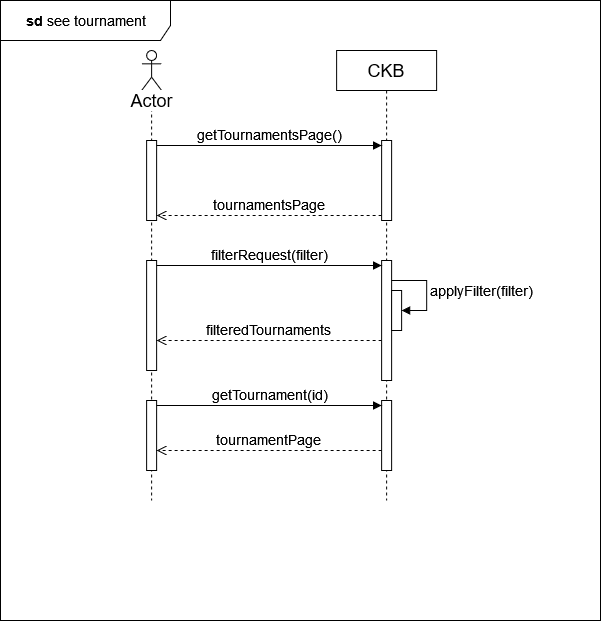
\includegraphics[width=\textwidth]{src/sequence_diagrams/tournaments.png}
    \end{figure}
}
{3}
{See tournament} % name
{User} % actor
{Registered user} % entry condition
{ % event flow
    \begin{enumerate}
        \item User requests to see the tournaments section
        \item The system shows the tournaments section
        \item User applies a filter (ongoing, finished, programming language)    
        \item The system shows the tournaments satisfying the filters
        \item User selects desired tournament
    \end{enumerate}
}
{The system shows the tournament page} % exit condition
{ % exceptions
    None
}
{ % notes
The tournament page displays all the information about that tournament, including rankings, battles and badges
}

\usecase
{
    \begin{figure}[H]
        \centering
        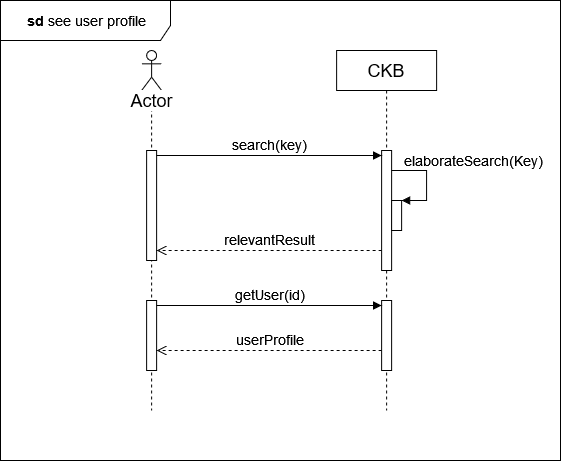
\includegraphics[width=\textwidth]{src/sequence_diagrams/userprofile.png}
    \end{figure}
}
{4}
{See user profile} % name
{User} % actor
{Registered user} % entry condition
{ % event flow
    \begin{enumerate}
        \item User searches a profile by name
        \item The system shows relevant results
        \item User selects the desired profile
    \end{enumerate}
}
{The system shows the profile page} % exit condition
{ % exceptions
    None
}
{ % notes
The profile page displays all the information about a profile, including badges if profile is a student's
}

\usecase
{
    \begin{figure}[H]
        \centering
        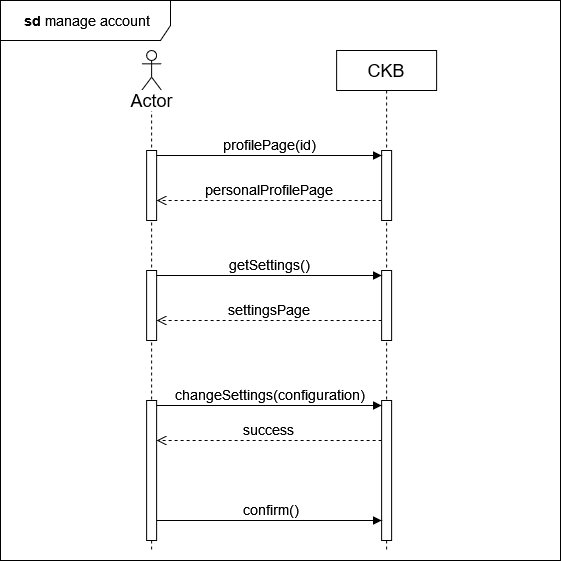
\includegraphics[width=\textwidth]{src/sequence_diagrams/manageaccount.png}
    \end{figure}
}
{5}
{Manage account} % name
{User} % actor
{Registered user} % entry condition
{ % event flow
    \begin{enumerate}
        \item User navigates to personal profile
        \item The system shows the personal profile page
        \item User selects 'change settings'
        \item The system shows the personal settings page
        \item User edits the personal settings to his liking, then clicks confirm
    \end{enumerate}
}
{The system saves the configurations} % exit condition
{ % exceptions
    \begin{itemize}
        \item None
    \end{itemize}
}
{ % notes

}


\usecase
{
    \begin{figure}[H]
        \centering
        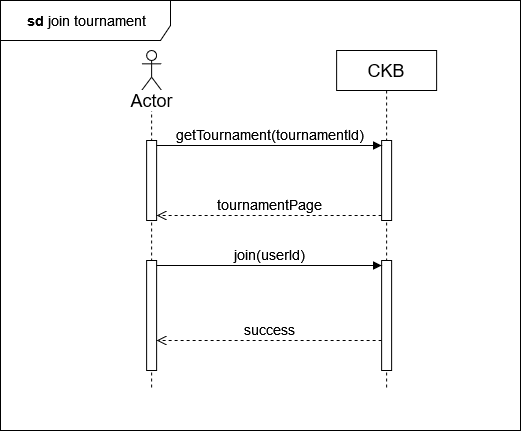
\includegraphics[width=\textwidth]{src/sequence_diagrams/jointourn.png}
    \end{figure}
}
{6}
{Join tournament} % name
{User} % actor
{User logged in to the platform as student, tournament still in subscription phase} % entry condition
{ % event flow
    \begin{enumerate}
        \item User requests the tournament page
        \item The system displays the tournament page
        \item User clicks the 'join' button
    \end{enumerate}
}
{User join the tournament} % exit condition
{ % exceptions
    \begin{itemize}
        \item None
    \end{itemize}
}
{ % notes

}

\usecase
{
    \begin{figure}[H]
        \centering
        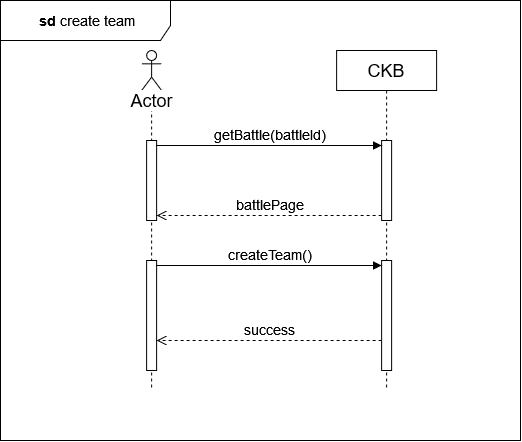
\includegraphics[width=\textwidth]{src/sequence_diagrams/createteam.png}
    \end{figure}
}
{7.1}
{Create team} % name
{User} % actor
{User logged in to the platform as Student, user subscribed to a tournament, the battle is related to that tournament and still in team formation phase, user is not yet part of a team} % entry condition
{ % event flow
    \begin{enumerate}
        \item User navigates to the battle page
        \item The system displays the battle page
        \item User clicks the create team button
    \end{enumerate}
}
{New team is created} % exit condition
{ % exceptions
    \begin{itemize}
        \item None
    \end{itemize}
}
{ % notes
None
}

\usecase
{
    \begin{figure}[H]
        \centering
        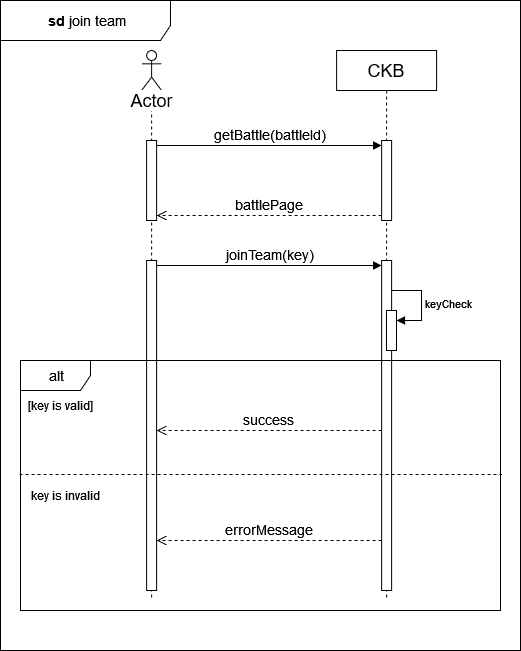
\includegraphics[width=\textwidth]{src/sequence_diagrams/jointeam.png}
    \end{figure}
}
{7.2}
{Join team} % name
{User} % actor
{User logged in to the platform as Student, user subscribed to a tournament, the battle is related to that tournament and still in team formation phase, user is not yet part of a team} % entry condition
{ % event flow
    \begin{enumerate}
        \item User navigates to the battle page
        \item The system displays the battle page
        \item User enters the team code
    \end{enumerate}
}
{User joins team} % exit condition
{ % exceptions
    \begin{itemize}
        \item Team code invalid
    \end{itemize}
}
{ % notes
    \begin{itemize}
        \item The system displays an error message
    \end{itemize}
}

\usecase
{
    \begin{figure}[H]
        \centering
        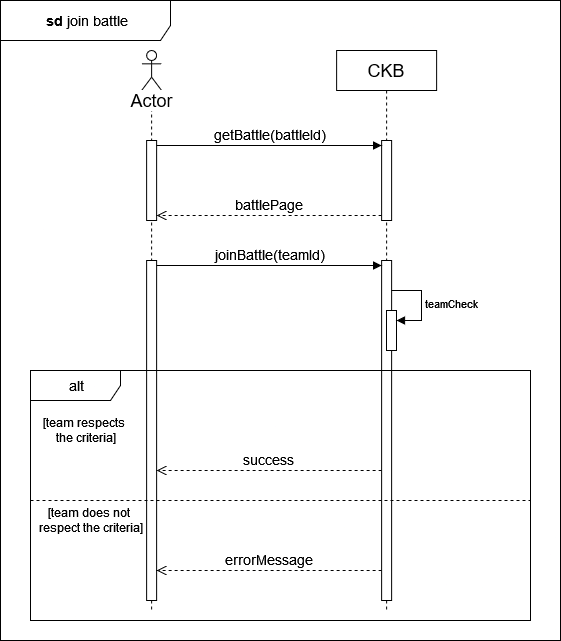
\includegraphics[width=\textwidth]{src/sequence_diagrams/joinbattle.png}
    \end{figure}
}
{7.3}
{Join battle} % name
{User} % actor
{User logged in to the platform as Student, User subscribed to a tournament, the battle is related to that tournament and still in team formation phase, User is the creator of a team} % entry condition
{ % event flow
    \begin{enumerate}
        \item User navigates to the battle page
        \item The system displays the battle page
        \item User clicks join battle
    \end{enumerate}
}
{The team user created joins the battle} % exit condition
{ % exceptions
    \begin{itemize}
        \item The team does not respect the minimum/maximum number of members per team criteria
    \end{itemize}
}
{ % notes
    \begin{itemize}
        \item The system displays an error message and asks to respect the criteria and try again
    \end{itemize}
}


\usecase
{
    {
    \begin{figure}[H]
        \centering
        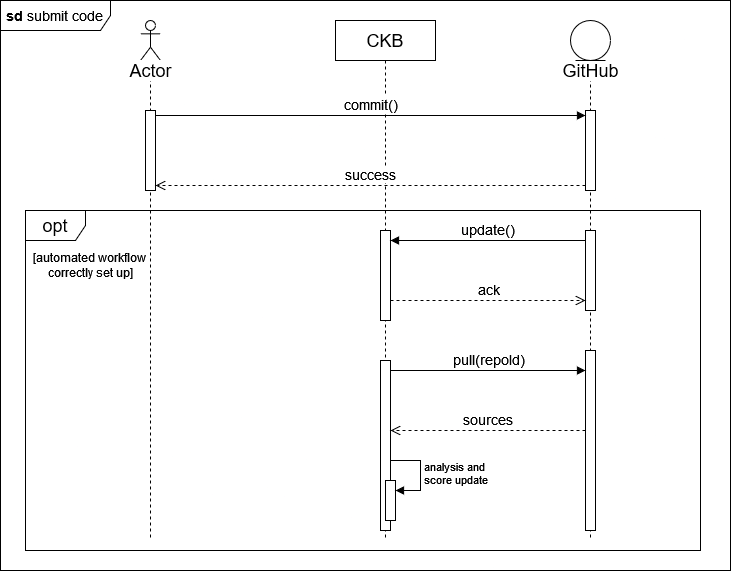
\includegraphics[width=\textwidth]{src/sequence_diagrams/submitcode.png}
    \end{figure}
}
}
{8}
{Submit code} % name
{User, GitHub} % actor
{User logged in to the platform as student, user joined a battle, battle is ongoing} % entry condition
{ % event flow
    \begin{enumerate}
        \item User commits code to main branch on GitHub
        \item GitHub notifies the System through an API call
        \item The system pulls the recent sources from GitHub and evaluates them
    \end{enumerate}
}
{The system shows the updated scores} % exit condition
{ % exceptions
    \begin{itemize}
        \item Student did not set up a proper automated workflow
    \end{itemize}
}
{ % notes
In case of exception, the system will not respond to the new push since It will not be notified
}

\usecase
{
    \begin{figure}[H]
        \centering
        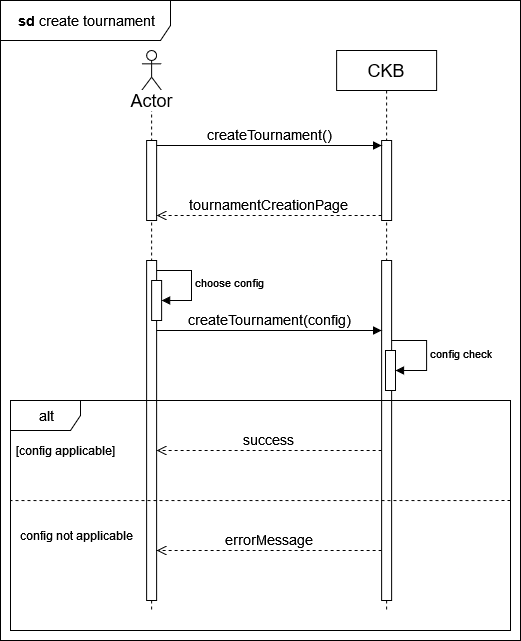
\includegraphics[width=\textwidth]{src/sequence_diagrams/createtourn.png}
    \end{figure}
}
{9}
{Create tournament} % name
{User} % actor
{User logged in to the platform as Educator} % entry condition
{ % event flow
    \begin{enumerate}
        \item User clicks the create tournament button
        \item The system shows the create torunament page
        \item User chooses his desired settings for that tournament, (including name, deadlines, badges, educators allowed to create battles, ...), then submits
    \end{enumerate}
}
{New tournament is created} % exit condition
{ % exceptions
    \begin{itemize}
        \item One or more of the settings is not applicable
    \end{itemize}
}
{ % notes
    \begin{itemize}
        \item Exception: the system displays a message showing the issue and asking to address It before trying again
    \end{itemize}
    User can choose his desired settings here, but he will be able to edit some of them even after tournament creation
}

\usecase
{
    \begin{figure}[H]
        \centering
        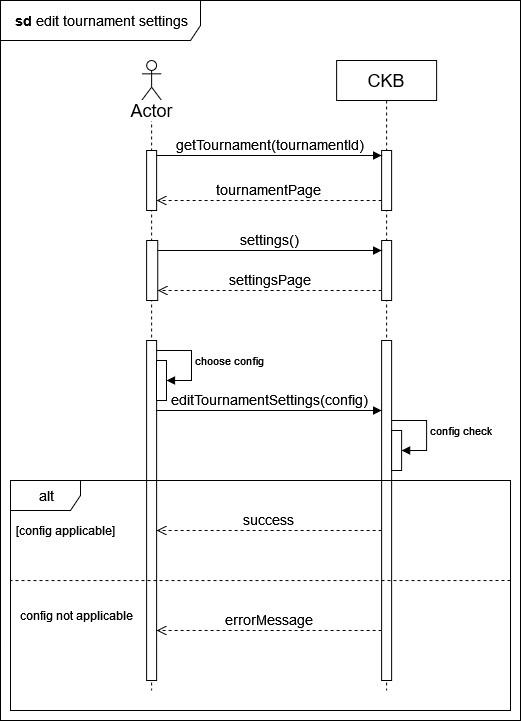
\includegraphics[width=\textwidth]{src/sequence_diagrams/managetournsetts.png}
    \end{figure}
}
{10}
{Edit tournament settings} % name
{User} % actor
{User logged in to the platform as educator, the tournament is not closed, user is the owner of the tournament} % entry condition
{ % event flow
    \begin{enumerate}
        \item User navigates to the tournament page
        \item The system shows the tournament page
        \item User goes to the settings section
        \item The system shows the settings page
        \item User chooses his desired settings, then submits
    \end{enumerate}
}
{Tournament settings are updated} % exit condition
{ % exceptions
    \begin{itemize}
        \item One or more of the settings is not applicable
    \end{itemize}
}
{ % notes
    \begin{itemize}
        \item Exception: the system displays a message showing the issue and asking to address It before trying again
    \end{itemize}
}

\usecase
{
    \begin{figure}[H]
        \centering
        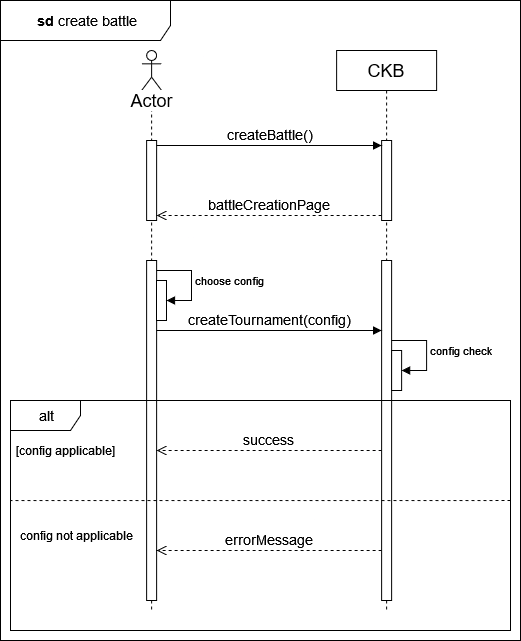
\includegraphics[width=\textwidth]{src/sequence_diagrams/createbattle.png}
    \end{figure}
}
{11.1}
{Create battle} % name
{User} % actor
{User logged in to the platform as educator, tournament is ongoing, user has been granted permission to create battles (or is the tournament creator itself)} % entry condition
{ % event flow
    \begin{enumerate}
        \item User navigates to the tournament page
        \item The system displays the tournament page
        \item User clicks the create new battle button
        \item The system shows the battle creation page
        \item User chooses his desired settings (like uploading code kata,            setting minimum and maximum number of students per team,                deadlines, ...) and submits
    \end{enumerate}
}
{New battle is created within the context of that tournament} % exit condition
{ % exceptions
    \begin{itemize}
        \item One or more of the settings is not applicable
    \end{itemize}
}
{ % notes
    \begin{itemize}
        \item Exception: the system displays a message showing the issue and asking to address It before trying again
    \end{itemize} 
    User can choose his desired settings here, but he will be able to edit some of them even after battle creation
}

\usecase
{
    \begin{figure}[H]
        \centering
        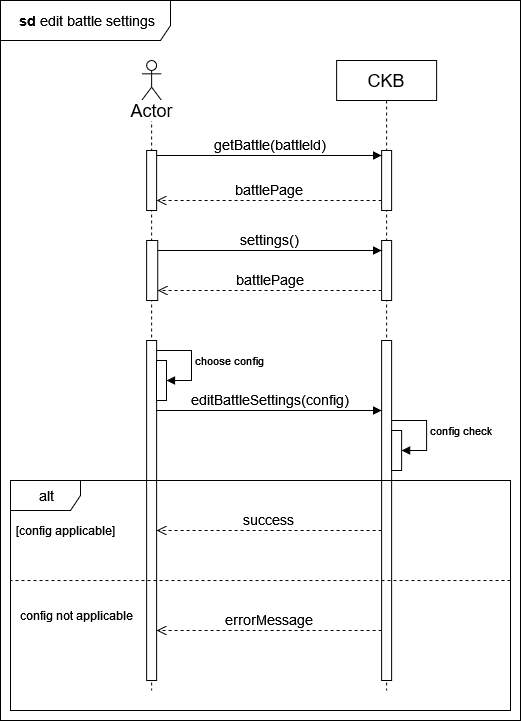
\includegraphics[width=\textwidth]{src/sequence_diagrams/managebattsetts.png}
    \end{figure}
}
{11.2}
{Edit battle settings} % name
{User} % actor
{User logged in to the platform as educator, battle is ongoing, user has been granted permission to create battles (or is the tournament creator itself)} % entry condition
{ % event flow
    \begin{enumerate}
        \item User navigates to the battle page
        \item User clicks the edit settings button
        \item The system shows the settings section
        \item User chooses his desired settings and submits
    \end{enumerate}
}
{Battle configurations are updated} % exit condition
{ % exceptions
    \begin{itemize}
        \item One or more of the settings is not applicable
    \end{itemize}
}
{ % notes
    \begin{itemize}
        \item Exception: the system displays a message showing the issue and asking to address It before trying again
    \end{itemize}
}

\usecase
{
    \begin{figure}[H]
        \centering
        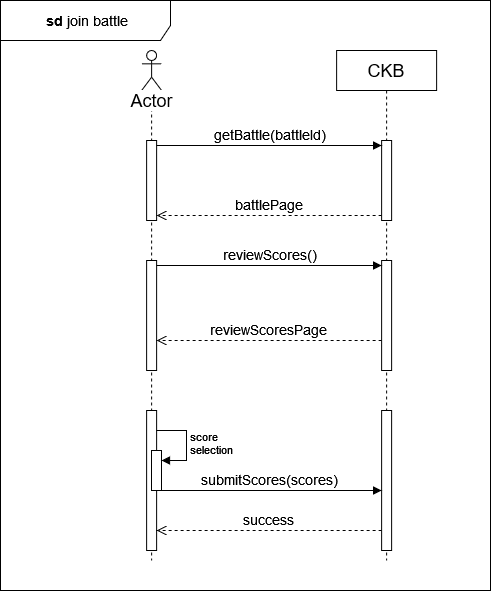
\includegraphics[width=\textwidth]{src/sequence_diagrams/revscores.png}
    \end{figure}
}
{11.3}
{Review scores} % name
{User} % actor
{User logged in to the platform as educator, battle is in consolidation phase, user has been granted permission to create battles (or is the tournament creator itself)} % entry condition
{ % event flow
    \begin{enumerate}
        \item User navigates to the battle page
        \item User clicks the review scores button
        \item The system shows the review scores section
        \item User performs manual evaluation, then submits
    \end{enumerate}
}
{Battle scores are updated} % exit condition
{ % exceptions
    \begin{itemize}
        \item None
    \end{itemize}
}
{ % notes

}

\usecase
{
    \begin{figure}[H]
        \centering
        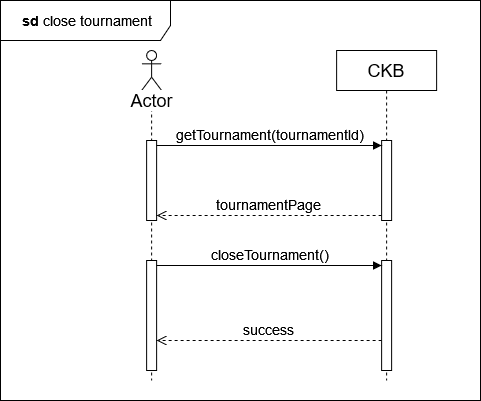
\includegraphics[width=\textwidth]{src/sequence_diagrams/closetourn.png}
    \end{figure}
}
{12}
{Close tournament} % name
{User} % actor
{User logged in to the platform as educator, tournament is ongoing, user is tournament creator} % entry condition
{ % event flow
    \begin{enumerate}
        \item User navigates to the tournament page
        \item The system shows the tournament page
        \item User clicks close tournament button
    \end{enumerate}
}
{Tournament is closed} % exit condition
{ % exceptions
    \begin{itemize}
        \item None
    \end{itemize}
}
{ % notes

}

\usecase
{
    \begin{figure}[H]
        \centering
        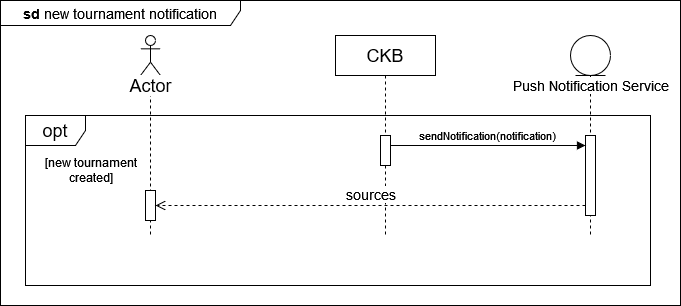
\includegraphics[width=\textwidth]{src/sequence_diagrams/pushtourn.png}
    \end{figure}
}
{13.1}
{New tournament notification} % name
{User, CKB Notification Service} % actor
{User logged in to the platform as student} % entry condition
{ % event flow
    \begin{enumerate}
        \item New tournament is created in the platform
        \item The system calls the CKB Notification Service
        \item CKB Notification Service sends the notification
    \end{enumerate}
}
{User is notified} % exit condition
{ % exceptions
    \begin{itemize}
        \item None
    \end{itemize}
}
{ % notes

}

\usecase
{
    \begin{figure}[H]
        \centering
        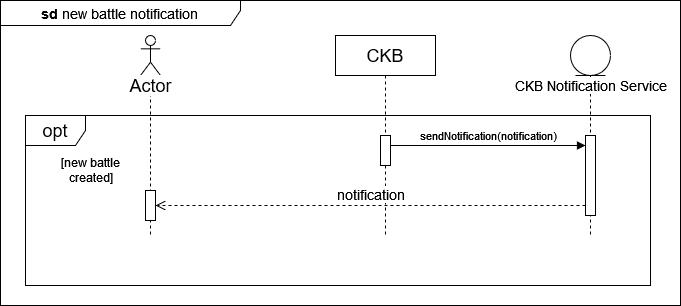
\includegraphics[width=\textwidth]{src/sequence_diagrams/notifybattle.png}
    \end{figure}
}
{13.2}
{New battle notification} % name
{User, CKB Notification Service} % actor
{User logged in to the platform as student, User subscribed to a tournament} % entry condition
{ % event flow
    \begin{enumerate}
        \item New battle is created in the context of a tournament user is subscribed to
        \item The system calls the CKB Notification Service
        \item CKB Notification Service sends the notification
    \end{enumerate}
}
{User is notified} % exit condition
{ % exceptions
    \begin{itemize}
        \item None
    \end{itemize}
}
{ % notes

}

\usecase
{
    \begin{figure}[H]
        \centering
        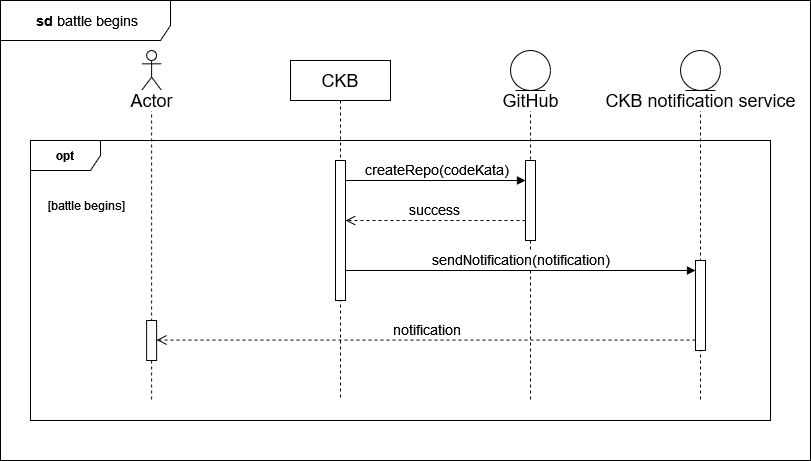
\includegraphics[width=\textwidth]{src/sequence_diagrams/battlebegins.png}
    \end{figure}
}
{13.3}
{Battle begins notification} % name
{User, CKB Notification Service, GitHub} % actor
{User logged in to the platform as student, User to a tournament, user joined a battle} % entry condition
{ % event flow
    \begin{enumerate}
        \item Battle team formation deadline expires, battle begins
        \item The system creates a new GitHub repository containing the codekata
        \item GitHub successfully creates the repository 
        \item The system calls the CKB Notification Service 
        \item CKB Notification Service sends the notification
    \end{enumerate}
}
{User receives the notification and the link to the github repository} % exit condition
{ % exceptions
    \begin{itemize}
        \item None
    \end{itemize}
}
{ % notes

}

